\documentclass[]{AVSSimReportMemo}
\usepackage{AVS}
\usepackage{colortbl}

\newcommand{\ModuleName}{singleAxisSpin}
\newcommand{\subject}{Guidance Module to Perform a Scanning over a Target}
\newcommand{\status}{Initial Version}
\newcommand{\preparer}{M. Cols}
\newcommand{\summary}{Generate the reference attitude trajectory to perform a scanning of a target. The initial pointing towards the target is assumed to be already achieved within the desired precision.}


\begin{document}


\makeCover


%
%	enter the revision documentation here
%	to add more lines, copy the table entry and the \hline, and paste after the current entry.
%
\pagestyle{empty}
{\renewcommand{\arraystretch}{2}
\noindent
\begin{longtable}{|p{0.5in}|p{4.5in}|p{1.14in}|}
\hline
{\bfseries Rev}: & {\bfseries Change Description} & {\bfseries By} \\
\hline
Draft & initial copy & M. Cols \\
\hline

\end{longtable}
}

\newpage
\setcounter{page}{1}
\pagestyle{fancy}

\tableofcontents
~\\ \hrule ~\\

\section{Module Input and Output}
Table \ref{tab:inputConfigTable} shows the input Configuration Data of the module Axis Scan.
\begin{table}[h!]
	\centering
	\caption{Input Configuration Data}
	\begin{tabular}{|l|l|l|p{3in}|}
		\hline
		\rowcolor{BrickRed}
		\textcolor{white}{Name} & \textcolor{white}{Type} & 
		\textcolor{white}{Length} & 
		\textcolor{white}{Description}  \\ \hline
		$\psi_0$ & double [] & 1 & 
		Third Euler Angle offset of the initial scanning frame $\mathcal{U}$ with respect the base input reference $\mathcal{R}_0$\\ \hline
		$\theta_0$& double [] & 1 & 
		Second Euler Angle offset of the initial scanning frame $\mathcal{U}$ with respect the base input reference $\mathcal{R}_0$\\ \hline
		$\dot{\psi}$ & double [] & 1 & 
		Third Euler Angle variation rate that defines the scanning motion  $\mathcal{R}$\\ \hline
	\end{tabular}
	\label{tab:inputConfigTable}
\end{table}

Table \ref{tab:inputRefTable} shows the initial Attitude Reference input message.
\begin{table}[h!]
	\centering
	\caption{Input Attitude Reference Message}
	\begin{tabular}{|l|l|l|p{3in}|}
		\hline
		\rowcolor{BrickRed}
		\textcolor{white}{Name} & \textcolor{white}{Type} & 
		\textcolor{white}{Length} & 
		\textcolor{white}{Description}  \\ \hline
		$\bm{\sigma}_{R_0/N}$ & double [] & 3 & 
		MRP attitude set of the input pointing frame with respect to the inertial frame. \\ \hline
		$\leftexp{N} {\bm{\omega}_{R_0/N}}$ & double [] & 3 & 
		Angular velocity of the input pointing frame with respect to the inertial frame expressed in inertial frame components. \\ \hline
		$\leftexp{N} {\bm{\dot{\omega}}_{R_0/N}}$ & double [] & 3 & 
		Angular acceleration of the input pointing frame with respect to the inertial frame expressed in inertial frame components. \\ \hline
	\end{tabular}
	\label{tab:inputRefTable}
\end{table}

Table \ref{tab:outputTable} shows the Attitude Reference output message of the module Axis Scan.
\begin{table}[h!]
	\centering
	\caption{Output Attitude Reference Message}
	\begin{tabular}{|l|l|l|p{3in}|}
		\hline
		\rowcolor{BrickRed}
		\textcolor{white}{Name} & \textcolor{white}{Type} & 
		\textcolor{white}{Length} & 
		\textcolor{white}{Description}  \\ \hline
		$\bm{\sigma}_{R/N}$ & double [] & 3 & 
		MRP attitude set of the desired reference frame with respect to the inertial frame. \\ \hline
		$\leftexp{N} {\bm{\omega}_{R/N}}$ & double [] & 3 & 
		Angular rate vector of the desired reference frame with respect to the inertial expressed in inertial frame components. \\ \hline
		$\leftexp{N} {\dot{\bm{\omega}}_{R/N}}$ & double [] & 3 & 
		Angular acceleration vector of the desired treference frame with respect to the inertial expressed in inertial frame components. \\ \hline
	\end{tabular}
	\label{tab:outputTable}
\end{table}
\newpage

\section{Introduction}
This technical note discusses the mathematics to compute a reference frame $\mathcal{R}$ that performs an horizontal scanning motion. From a state of accurate pointing towards a desired target, $\mathcal{R}_0$ , the present module receives the pointing frame information and applies a constant offset correction in orientation to relocate the pointing axis where the scanning motion is to be initiated. Figure~\ref{fig:fig1} shows the correlation between the target pointing reference $\mathcal{R}_0$ and the initial scanning reference $\mathcal{U}$. The offset correction is determined by the second and third angles of an 123-Euler attitude set ($\theta_0$ and $\psi_0$ respectively). Once the scanning axis initial pointing has been stabilized, an horizontal scanning motion is performed until the maneuver time is finished.
\begin{figure}[htb]
	\centerline{
	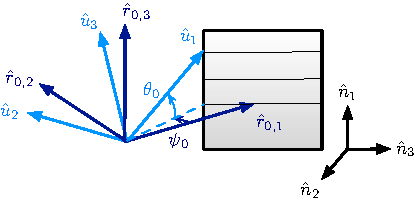
\includegraphics{Figures/fig1}
	}
	\caption{Illustration of the input pointing frame $\mathcal{R}_{0}:\{ \hat {\bm r}_{0,1}, \hat {\bm r}_{0,2}, \hat {\bm r}_{0,3} \}$,
	the initial scanning frame $\mathcal{U}:\{ \hat {\bm u}_{1}, \hat {\bm u}_{2}, \hat {\bm u}_{3} \}$
	 and the inertial frame $\mathcal{N}:\{ \hat{\bm n}_{1}, \hat{\bm n}_{2}, \hat{\bm n}_{3} \}$.}
	\label{fig:fig1}
\end{figure}

\section{Scanning Frame Initialization}
For the sake of robustness, the transformation from the input reference $\mathcal{R}_0$ to the initial scanning reference  $\mathcal{U}$ is achieved through the addition property of Direction Cosine Matrices, aka DCMs. 
Reference $\mathcal{U}$ can be obtained by applying two consecutive rotations on $\mathcal{R}_0$. The first rotation of angle  $\psi_0$ is about the third axis of the base frame, $\hat {\bm r}_{0,3}$. The second rotation of angle $\theta_0$ is about the second axis of the resulting frame, $\hat {\bm u}_{0,2}$. Such relationship can be expressed as following:
\begin{equation}
	[UN] = [M_2( \theta_0)][M_3(\psi_0)][R_{0}N]
\end{equation}
Where
\begin{equation}
  [M_3(\psi_0)] =  
  	\begin{bmatrix}
    		\cos\psi_0 & -\sin\psi_0 & 0 \\
    		\sin\psi_0 & \cos\psi_0 &0 \\
    		0 & 0 & 1
	\end{bmatrix}
\end{equation}
\begin{equation}
  [M_2(\theta_0)] =  
  	\begin{bmatrix}
  		\cos\theta_0 & 0 & -\sin\theta_0  \\
    		0 & 1 & 0 \\
    		\sin\theta_0 & 0 & \cos\theta_0  
	\end{bmatrix}
\end{equation}

Making use of the Rigid Body Kinematics library of Reference~\citenum{schaub}, the conversion from the input MRP attitude set $\bm{\sigma}_{R_{0}N}$ to its corresponding DCM is achieved and the Euler Angle rotation matrices are computed. 
\begin{equation}
	[R_{0}N] = \textrm{MRP2C}(\bm{\sigma}_{R_{0}N})
\end{equation}
\begin{equation}
	[M_2] = \textrm{ Mi}(\theta_0, 2)
\end{equation}
\begin{equation}
	[M_3] =\textrm{ Mi}(\psi_0, 3)
\end{equation}
Where the first parameter of the $\textrm{ Mi}$ function is the rotated Euler Angle and the second parameter is the index of the axis about which the rotation is performed.

Eventually, the MRP attitude set of the initial scanning frame is obtained:
\begin{equation}
	\bm{\sigma}_{U/N} =  \textrm{C2MRP}([UN])
\end{equation}


\section{Reference Frame Generation}
\begin{figure}[htb]
	\centerline{
	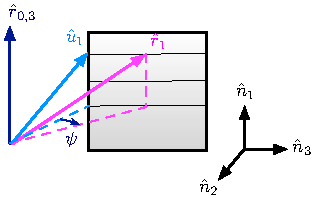
\includegraphics{Figures/fig2}
	}
	\caption{Illustration of the initial scanning axis $\hat {\bm u}_1$
	 and the time-varying scanning axis $\hat{\bm r}_1(t)$.}
	\label{fig:fig2}
\end{figure}

\subsection{Angular Rates and Acceleration}
Since the initial scanning axis $\hat{\bm u}_1$ differs from the input pointing reference $\hat{\bm r}_{0,1}$ in a constant offset, the relative angular rate and acceleration of $\mathcal{U}$ with respect to  $\mathcal{R}_0$ are zero,
$$  \bm{\omega}_{U/R_{0}} = \dot{\bm{\omega}}_{U/R_{0}} = \bm{0}$$  
In turn, the motion of the current scanning frame  $\mathcal{R}$  with respect the initial scanning frame $\mathcal{U}$ can be expressed as a negative rotation of angle $\psi =\dot{\psi}t$ about $\hat {\bm r}_{0,3}$.
\begin{equation}
	\bm{\omega}_{R/U} =  
	\leftexp{R_{\textrm{0}}} {\begin{bmatrix} 0 \\ 0 \\  -\dot\psi \end{bmatrix}}
\end{equation}
As seen by the input pointing frame $\mathcal{R}_0$, the scanning angular velocity is constant. Thus,
\begin{equation}
	\dot{\bm{\omega}}_{R/U} =  
	\leftexp{R_{\textrm{0}}} {\begin{bmatrix} 0 \\ 0 \\  0 \end{bmatrix}}
\end{equation}
The angular velocity of the reference with respect to the inertial in inertial frame components is straightly computed:
\begin{subequations} 
	\begin{equation}
		\leftexp{N} {\bm{\omega}_{R/N}} = \leftexp{N} {\bm{\omega}_{R/U}} +  \leftexp{N} {\bm{\omega}_{U/R_0}} +   \leftexp{N} {\bm{\omega}_{R_{0}/N}}
	\end{equation}
	\begin{equation}
		\leftexp{N} {\bm{\omega}_{R/N}} =  [R_{0}N]^{T} \textrm{ } \leftexp{R_{\textrm{0}}}{\bm{\omega}_{R/U}}  +   \leftexp{N} {\bm{\omega}_{R_{0}/N}}
	\end{equation}
\end{subequations}

Similarly, for the angular acceleration:
\begin{subequations}
	\begin{equation}
		\leftexp{N} {\dot{\bm{\omega}}_{R/N}} = \leftexp{N} {\dot{\bm{\omega}}_{R/U}} +  \leftexp{N} {\dot{\bm{\omega}}_{U/R_0}} +   \leftexp{N} {\dot{\bm{\omega}}_{R_{0}/N}}
	\end{equation}
	\begin{equation}
		\leftexp{N} {\dot{\bm{\omega}}_{R/N}} = [R_{0}N]^{T} \textrm{ } \leftexp{R_{\textrm{0}}}{\dot{\bm{\omega}}_{R/U}} +   \leftexp{N} {\dot{\bm{\omega}}_{R_{0}/N}}
	\end{equation}
\end{subequations}
Where $\dot{\bm{\omega}}_{R/U}$ is obtained using the Transport Theorem:
\begin{subequations}
	\begin{equation}
		\dot{\bm{\omega}}_{R/U} = 
		 \leftexp{R_{\textrm{0}}} {\frac{\textrm{d}}{\textrm{dt}}} \bm{\omega}_{R/U}  + \bm\omega_{R_{0}/N} \times  \bm\omega_{R/U}
	\end{equation}
	\begin{equation}
		\dot{\bm{\omega}}_{R/U} =  \bm\omega_{R_{0}/N} \times  \bm\omega_{R/U}
	\end{equation}
\end{subequations}

\subsection{Attitude}
As depicted in Figure~\ref{fig:fig2}, the current position of the scanning axis $\hat{\bm{r}}_1$ can be tracked in analogy with how $\mathcal{U}$ was computed in the initialization process:
\begin{equation}
	[RN] = [M_2( \theta_0)][M_3(\psi)][R_{0}N]
\end{equation}
Where 
\begin{equation}
	\psi = \psi_0 - \dot\psi t
\end{equation}

Eventually, the corresponding MRP set is computed:
\begin{equation}
	\bm{\sigma}_{R/N} =  \textrm{C2MRP}([RN])
\end{equation}

\bibliographystyle{unsrt}
\bibliography{references}

\end{document}
